% Informe del TP5 del equipo de la señal 2.
% Preámbulo común de los informes del TP5 (señal 1 y señal 2), con el estilo de los trabajos anteriores.
\documentclass[12pt]{article}
\usepackage[utf8]{inputenc}
\usepackage[T1]{fontenc}
\usepackage{graphicx}
\usepackage[spanish,es-tabla]{babel}
\usepackage{amsmath}
\usepackage{amssymb}
\usepackage[a4paper,margin=1in]{geometry}
\usepackage{subcaption}
\usepackage{mathtools}
\usepackage[table,xcdraw]{xcolor}
\usepackage[style=ieee, backend=bibtex]{biblatex}
\usepackage{enumitem}
\usepackage{array}
\usepackage{longtable}
\usepackage{multirow}
\usepackage{booktabs}
\usepackage{csquotes}
\usepackage{tikz}
\usetikzlibrary{arrows.meta, positioning, shapes.geometric, babel}
\usepackage[hidelinks]{hyperref}
\usepackage{float}
\usepackage{setspace}
\onehalfspacing
\graphicspath{{Figuras/}}

\addbibresource{bibliografia.bib}
\hypersetup{colorlinks=true, linkcolor=blue, citecolor=blue, urlcolor=blue, filecolor=blue}

% Portada: \portada{integrantes (tabla)}{señal}
\newcommand{\portada}[2]{%
\begin{titlepage}
\thispagestyle{empty}
\begin{tikzpicture}[remember picture,overlay]
    \node[opacity=0.2,anchor=center] at (current page.center)
        {
\includegraphics[width=0.9\paperwidth]{decoracion_a.png}};
\end{tikzpicture}
\begin{center}
    
\includegraphics[width=15cm]{unc_fcefyn_logo.png} \\ [0.5cm]
    \LARGE Universidad Nacional de Córdoba \\ [0.5cm]
    \large Facultad de Ciencias Exactas, Físicas y Naturales \\
    \vspace{40pt}
    \large Sistemas de Radiocomunicación \\ [0.2cm]
    \large Trabajo Práctico N.° 5 \\
    \vspace{50pt}
    \LARGE Radar \\[0.3cm]
    \large Procesamiento de la señal #2 \\
    \vspace{50pt}
    \begin{table}[!h]
        \centering
        \begin{tabular}{ll}
            \multicolumn{1}{c}{Nombre} & \multicolumn{1}{c}{DNI} \\
            #1
        \end{tabular}
    \end{table}
    \vspace{20pt}
    \begin{table}[!h]
        \centering
        \begin{tabular}{ll}
            \multicolumn{1}{c}{Docentes} & Esp. Ing. Liendo, Carlos Guillermo \\
                                         & Ing. Dadam, Federico Tomás \\
        \end{tabular}
    \end{table}
    \vfill
        {\small Córdoba, República Argentina\\ Año 2026}
\end{center}
\end{titlepage}
}

\newcommand{\senal}{2}
\newcommand{\figdir}{senal_2}

\begin{document}
\renewcommand{\figureautorefname}{Fig.}
\renewcommand{\tableautorefname}{Tab.}
\renewcommand{\equationautorefname}{Ec.}

\portada{Mendes Rosa, Agustín & 44.517.201 \\ Monja, Ernesto Joaquín & 43.873.728 \\}{2}
\newpage
\tableofcontents
\newpage
\listoffigures
\newpage

\section{Introducción}
El presente informe desarrolla la Actividad 5 de Sistemas de Radiocomunicación, dedicada al radar \cite{consigna}. En la parte teórica se definen el radar y sus aplicaciones, la ecuación del radar y los conceptos de detección, la sección radar (RCS), el filtro apareado, el clutter y la señal chirp con su compresión, sobre la base del material de la cátedra \cite{apunte} y de la bibliografía indicada \cite{skolnik, richards, cumming}.

En la parte práctica se procesa la señal \senal{} asignada al equipo: una detección simulada de radar de 100 pulsos con entre 2 y 10 blancos de rangos y velocidades desconocidos. Se implementaron la compresión con filtro apareado, la ventana CFAR, los canceladores MTI simple, STI simple y MTI doble y el filtrado Doppler, y con ellos se determinaron el rango y la velocidad de cada blanco.

% !TEX root = ../informe_senal1.tex
\section{Parte teórica}
\label{sec:teorico}

% =====================================================================
\subsection{El radar: definición, usos, parámetros y diagrama en bloques}
\label{sec:radar}

RADAR es el acrónimo de \textit{RAdio Detection And Ranging}: un sistema que irradia ondas electromagnéticas y analiza los ecos que devuelven los objetos (blancos) para detectarlos y estimar su posición y su movimiento \cite{skolnik, apunte}. La distancia $R$ se obtiene del tiempo de ida y vuelta $\Delta t$ del eco, según la ecuación \ref{eq:dist}:

\begin{equation}
    R = \frac{c \, \Delta t}{2}
    \label{eq:dist}
\end{equation}

$R = c \, \Delta t / 2$. La dirección surge del apuntamiento de la antena, y la velocidad radial, del corrimiento Doppler $f_D = 2 v_r / \lambda$. Como usa su propia iluminación, el radar funciona de día y de noche y a través de nubes, niebla y lluvia, a distancias mucho mayores que los sensores ópticos.

\textbf{Usos.} Se emplea en aplicaciones civiles y militares \cite{skolnik}:
\begin{itemize}
    \item \underline{Control de tránsito aéreo:} vigilancia de ruta y de aproximación, radar secundario y de superficie de aeropuertos.
    \item \underline{Meteorología:} detección de precipitaciones y medición de vientos por Doppler.
    \item \underline{Navegación:} radares marítimos anticolisión, altímetros y radares de navegación de aeronaves.
    \item \underline{Defensa:} vigilancia, seguimiento de misiles, control de tiro y guiado.
    \item \underline{Observación de la Tierra:} radares de apertura sintética (SAR) satelitales, como los SAOCOM de la CONAE, en banda L.
    \item \underline{Otros:} radares automotrices de asistencia a la conducción, cinemómetros, radar de penetración terrestre y radioastronomía.
\end{itemize}

\textbf{Parámetros típicos de trabajo.} La frecuencia, la potencia, la forma de onda y la PRF dependen de la aplicación. Las frecuencias bajas (bandas L y S) tienen menos atenuación atmosférica y permiten antenas grandes y alcances largos; las altas (X, Ku, Ka) dan mayor resolución angular con antenas chicas, pero sufren más atenuación por lluvia \cite{skolnik, apunte}. La \autoref{tab:radares} resume valores representativos.

\begin{table}[H]
    \centering
    \footnotesize
    \caption{Parámetros típicos de radares según la aplicación \cite{skolnik, richards}.}
    \label{tab:radares}
    \begin{tabular}{|p{3.4cm}|p{2.6cm}|p{2.8cm}|p{2.4cm}|p{3.0cm}|}
        \hline
        \textbf{Aplicación} & \textbf{Banda / frecuencia} & \textbf{Potencia} & \textbf{PRF} & \textbf{Alcance} \\
        \hline
        Vigilancia aérea de ruta & L (1,2--1,4 GHz) & Pico de 1 a 5 MW & 300 a 400 Hz & 200 a 400 km \\
        \hline
        Vigilancia de aproximación (ASR) & S (2,7--2,9 GHz) & Pico $\approx$ 1 MW & $\approx$ 1 kHz & $\approx$ 100 km \\
        \hline
        Meteorológico (WSR-88D) & S (2,7--3,0 GHz) & Pico de 750 kW & 318 a 1304 Hz & Hasta 460 km \\
        \hline
        Navegación marítima & X (9,4 GHz) y S & Pico de 10 a 25 kW & 1 a 3 kHz & 50 a 100 km \\
        \hline
        Control de tiro y seguimiento & X, Ku & Pico de decenas a cientos de kW & Media a alta (10--200 kHz) & 10 a 100 km \\
        \hline
        Automotriz (FMCW) & W (76--81 GHz) & Del orden de 10 mW & Barrido continuo & Hasta 250 m \\
        \hline
        SAR satelital & L (SAOCOM), C, X & Pico de kW & 1 a 5 kHz & Cientos de km (franjas de decenas de km) \\
        \hline
        Este trabajo práctico & L (1,3 GHz) & -- & 1500 Hz & Ventana de 30 km \\
        \hline
    \end{tabular}
\end{table}

\textbf{Diagrama en bloques.} La \autoref{fig:bloques} muestra el diagrama de un radar pulsado típico, basado en el del apunte de la cátedra \cite{apunte} y en Skolnik \cite{skolnik}.

\begin{figure}[H]
    \centering
    \resizebox{\textwidth}{!}{%
    \begin{tikzpicture}[font=\footnotesize, node distance=0.6cm and 0.9cm,
        bloque/.style={draw, thick, rounded corners=2pt, fill=blue!8, minimum height=1.0cm, text width=2.3cm, align=center},
        flecha/.style={-{Stealth}, thick}]
        \node[bloque] (gen) {Generador de forma de onda};
        \node[bloque, right=of gen] (mod) {Modulador de pulsos};
        \node[bloque, right=of mod] (pa) {Amplificador de potencia};
        \node[bloque, right=of pa, fill=orange!15] (dup) {Duplexor};
        \node[right=1.2cm of dup] (ant) {\Large$\Psi$};
        \node[above=0.05cm of ant, font=\scriptsize] {Antena};
        \node[bloque, below=1.3cm of dup] (lna) {Amplificador de bajo ruido};
        \node[bloque, left=of lna] (mix) {Mezclador};
        \node[bloque, above=0.5cm of mix, fill=green!10] (ol) {Oscilador local};
        \node[bloque, left=of mix] (fi) {Amplificador de FI y filtro apareado};
        \node[bloque, left=of fi] (det) {Detector (demodulador I/Q)};
        \node[bloque, below=1.0cm of det, fill=purple!10] (proc) {Procesador de señal: MTI, Doppler, CFAR};
        \node[bloque, right=of proc, fill=purple!10] (datos) {Procesador de datos: detección y seguimiento};
        \node[bloque, right=of datos] (disp) {Presentación (display)};
        \node[bloque, below=0.4cm of gen, fill=yellow!20] (sinc) {Sincronizador (PRF)};
        \draw[flecha] (gen) -- (mod); \draw[flecha] (mod) -- (pa); \draw[flecha] (pa) -- (dup);
        \draw[{Stealth}-{Stealth}, thick] (dup) -- (ant);
        \draw[flecha] (dup) -- (lna); \draw[flecha] (lna) -- (mix); \draw[flecha] (ol) -- (mix);
        \draw[flecha] (mix) -- (fi); \draw[flecha] (fi) -- (det); \draw[flecha] (det) -- (proc);
        \draw[flecha] (proc) -- (datos); \draw[flecha] (datos) -- (disp);
        \draw[flecha, dashed] (sinc) -- (gen);
        \draw[flecha, dashed] (sinc.south) |- (proc.west);
    \end{tikzpicture}}
    \caption{Diagrama en bloques de un radar pulsado típico. Elaboración propia a partir de \cite{apunte, skolnik}.}
    \label{fig:bloques}
\end{figure}

\begin{itemize}
    \item \underline{Sincronizador:} genera la temporización de todo el sistema, es decir, la PRF y las ventanas de recepción.
    \item \underline{Generador de forma de onda y modulador:} generan el pulso a transmitir (por ejemplo, un chirp) y lo encienden y apagan según la PRF.
    \item \underline{Amplificador de potencia:} eleva el pulso a la potencia pico de transmisión (magnetrón, klistrón, tubo de onda progresiva o amplificadores de estado sólido).
    \item \underline{Duplexor:} conmuta la antena entre el transmisor y el receptor y protege al receptor durante la transmisión. Por eso existe un rango mínimo, con el receptor ciego mientras dura el pulso y el tiempo de recuperación.
    \item \underline{Antena:} concentra la energía en un haz angosto, que da la ganancia y la resolución angular, y capta los ecos.
    \item \underline{Amplificador de bajo ruido (LNA):} fija la figura de ruido del sistema.
    \item \underline{Mezclador y oscilador local:} trasladan la señal a frecuencia intermedia o a banda base.
    \item \underline{Amplificador de FI y filtro apareado:} amplifican y maximizan la relación señal a ruido. Con formas de onda moduladas, el filtro apareado realiza la compresión del pulso.
    \item \underline{Detector:} obtiene la envolvente o las componentes en fase y cuadratura (I/Q), que conservan la fase para el procesamiento Doppler.
    \item \underline{Procesador de señal:} cancela el clutter (MTI), separa los blancos por velocidad (filtrado Doppler), integra pulsos y decide la presencia de blancos con un umbral adaptativo (CFAR).
    \item \underline{Procesador de datos y presentación:} asocian detecciones, estiman trayectorias y muestran la situación al operador.
\end{itemize}

% =====================================================================
\subsection{Ecuación del radar, ruido y detección}
\label{sec:ecuacion}

\textbf{Ecuación del radar.} Un radar monoestático que transmite una potencia pico $P_t$ con una antena de ganancia $G$ produce sobre un blanco a distancia $R$ una densidad de potencia $P_t G / (4\pi R^2)$. El blanco intercepta y reirradia isotrópicamente la potencia que incide sobre su sección radar $\sigma$; el eco vuelve a dispersarse en $4\pi R^2$ y lo capta la apertura efectiva $A_e = G\lambda^2/(4\pi)$ \cite{skolnik, apunte}:
\begin{equation}
    P_r = \frac{P_t \, G}{4\pi R^2} \cdot \frac{\sigma}{4\pi R^2} \cdot \frac{G \lambda^2}{4\pi} \cdot \frac{1}{L} = \frac{P_t \, G^2 \lambda^2 \sigma}{(4\pi)^3 R^4 L}
    \label{eq:radar}
\end{equation}
\begin{itemize}
    \item $P_t$: potencia pico transmitida [W]; $G$: ganancia de la antena; $\lambda$: longitud de onda [m].
    \item $\sigma$: sección radar (RCS) del blanco [m$^2$] (\autoref{sec:rcs}).
    \item $R$: distancia al blanco [m]. El factor $R^{-4}$ refleja la doble dispersión esférica: duplicar el alcance exige 16 veces más potencia.
    \item $L \geq 1$: pérdidas totales (líneas, radomo, forma del haz, procesamiento, propagación atmosférica).
\end{itemize}

\textbf{Efecto del ruido.} El eco compite con el ruido del receptor, de potencia $N = k T_s B_n$, con $k$ la constante de Boltzmann, $T_s$ la temperatura de ruido del sistema (antena, línea y receptor) y $B_n$ el ancho de banda de ruido. La relación señal a ruido es
\begin{equation}
    SNR = \frac{P_t \, G^2 \lambda^2 \sigma}{(4\pi)^3 R^4 \, k T_s B_n L},
    \qquad
    R_{max} = \left[ \frac{P_t \, G^2 \lambda^2 \sigma}{(4\pi)^3 \, k T_s B_n L \, SNR_{min}} \right]^{1/4}
    \label{eq:snr}
\end{equation}
donde $SNR_{min}$ es la relación mínima para detectar con las probabilidades exigidas. El ruido es aleatorio: el detector compara la envolvente de la señal con un umbral $V_T$, y tanto el ruido solo como el blanco más ruido pueden quedar de uno u otro lado. Por eso la detección es un problema estadístico \cite{richards}.

\textbf{Probabilidad de falsa alarma y de detección.} Con ruido gaussiano complejo de potencia $\psi_0$, la envolvente del ruido tiene distribución de Rayleigh y la probabilidad de que supere el umbral sin que haya blanco es \cite{skolnik, richards}
\begin{equation}
    P_{fa} = \int_{V_T}^{\infty} \frac{r}{\psi_0} e^{-r^2/2\psi_0} \, dr = e^{-V_T^2 / 2\psi_0}
\end{equation}
La \textbf{probabilidad de falsa alarma} $P_{fa}$ es, entonces, la probabilidad de declarar un blanco donde solo hay ruido; fija el umbral, y se expresa también como tiempo medio entre falsas alarmas $T_{fa} \approx 1/(P_{fa} B_n)$. La \textbf{probabilidad de detección} $P_d$ es la probabilidad de que la envolvente del blanco más ruido (distribución de Rice) supere ese umbral; aumenta con la SNR. Para un blanco no fluctuante, $P_d = 0{,}9$ con $P_{fa} = 10^{-6}$ requiere una SNR de unos $13{,}2 \, [dB]$ en un solo pulso \cite{apunte}, valor que reproduce la aproximación de Albersheim. Si la RCS fluctúa (modelos de Swerling), la SNR necesaria es mayor.

\textbf{Integración de pulsos.} El radar recibe varios ecos del mismo blanco durante el tiempo de iluminación, y combinarlos reduce la SNR necesaria por pulso \cite{apunte, richards}:
\begin{itemize}
    \item \underline{Integración coherente:} suma las muestras complejas (amplitud y fase) de $n$ pulsos. Las señales se suman en fase y el ruido, independiente entre pulsos, en potencia, por lo que la SNR crece $n$ veces: $SNR_n = n \cdot SNR_1$. Requiere conocer la fase, es decir, compensar el Doppler (por ejemplo, con la FFT del procesamiento Doppler).
    \item \underline{Integración no coherente:} suma las envolventes, después del detector. Pierde la fase, pero es más simple; su ganancia es menor que $n$, del orden de $n^{0{,}7}$ a $n^{0{,}8}$ para $n$ grande, y se expresa con una eficiencia de integración $E_i(n) < 1$.
\end{itemize}
En la ecuación del radar, la integración de $n$ pulsos divide por $n E_i(n)$ la SNR mínima de un pulso (con $E_i = 1$ para la integración coherente):
\begin{equation}
    R_{max} = \left[ \frac{P_t \, G^2 \lambda^2 \sigma \, n E_i(n)}{(4\pi)^3 \, k T_s B_n L \, SNR_1} \right]^{1/4}
\end{equation}
por lo que el alcance aumenta en $(n E_i)^{1/4}$.

% =====================================================================
\subsection{Sección radar (RCS)}
\label{sec:rcs}

\textbf{Definición.} La sección radar $\sigma$ es el área ficticia que, interceptando la potencia incidente y reirradiándola isotrópicamente, produciría en el radar el mismo eco que el blanco real \cite{apunte, skolnik}:
\begin{equation}
    \sigma = \lim_{R \to \infty} 4\pi R^2 \frac{|E_s|^2}{|E_i|^2} \quad [m^2]
\end{equation}
donde $E_i$ es el campo incidente en el blanco y $E_s$ el campo dispersado hacia el radar. No coincide con el área física: depende de la frecuencia, la polarización, la forma, el material, la orientación y la geometría monoestática o biestática. Se expresa también en dBsm (dB respecto de 1 m$^2$). Valores típicos van de $10^{-5}$ m$^2$ (insectos) a 1 m$^2$ (un avión liviano), 100 m$^2$ (un avión de pasajeros grande) y $10^4$ m$^2$ (un buque) \cite{apunte}.

\textbf{Esfera conductora.} Es el blanco de referencia, porque su RCS no depende del ángulo de observación. Su comportamiento con la frecuencia, que se obtiene con la serie de Mie, tiene tres regiones (\autoref{fig:rcs_esfera}) \cite{skolnik}:
\begin{itemize}
    \item \underline{Región de Rayleigh} ($ka = 2\pi a/\lambda \ll 1$): $\sigma \approx 9\pi a^2 (ka)^4$, proporcional a $f^4$. Por eso las gotas de lluvia y los insectos reflejan mucho más en frecuencias altas.
    \item \underline{Región de resonancia o de Mie} ($ka \approx 1$ a $10$): la RCS oscila por la interferencia entre la reflexión especular y la onda que rodea la esfera (onda de arrastre). El máximo, cerca de $ka = 1$, es unas 3,6 veces el área geométrica.
    \item \underline{Región óptica} ($ka \gg 1$): $\sigma \to \pi a^2$, el área de la sección transversal.
\end{itemize}

\begin{figure}[H]
    \centering
    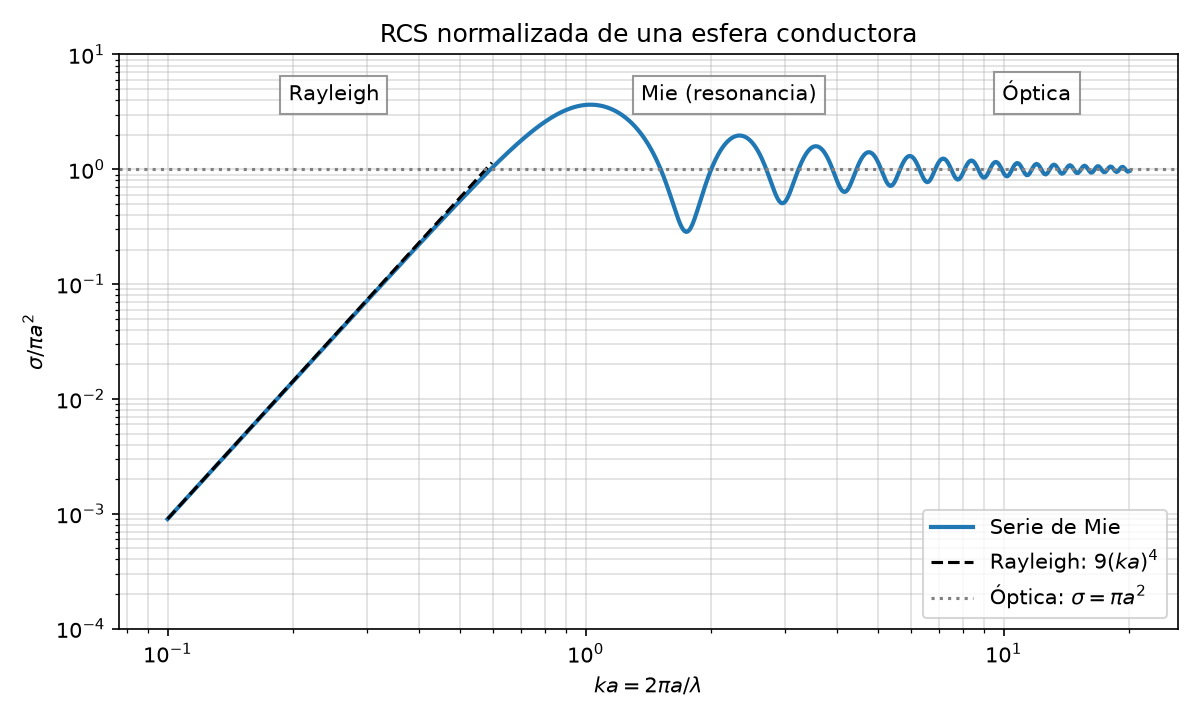
\includegraphics[width=0.8\textwidth]{teoria/rcs_esfera.png}
    \caption{RCS normalizada de una esfera conductora en función de su tamaño eléctrico, calculada con la serie de Mie. Elaboración propia.}
    \label{fig:rcs_esfera}
\end{figure}

\textbf{Placa plana.} Como segundo blanco simple se elige una placa plana conductora de área $A$. Con incidencia normal se comporta como un espejo y su RCS es muy grande, $\sigma_{max} = 4\pi A^2/\lambda^2$. Fuera de la normal, la reflexión especular se aleja del radar y la RCS cae según un diagrama del tipo $\left[\sin(kL\sin\theta)/(kL\sin\theta)\right]^2$, con un lóbulo principal angosto ($\approx \lambda/L$) \cite{skolnik}. La \autoref{fig:rcs_placa} muestra una placa de $1 \times 1$ m a 10 GHz: en la normal alcanza $41{,}4$ dBsm (unos $14.000$ m$^2$), pero a pocos grados cae más de 30 dB. Este es el principio de las aeronaves de baja observabilidad, que orientan sus superficies planas lejos de las direcciones de los radares.

\begin{figure}[H]
    \centering
    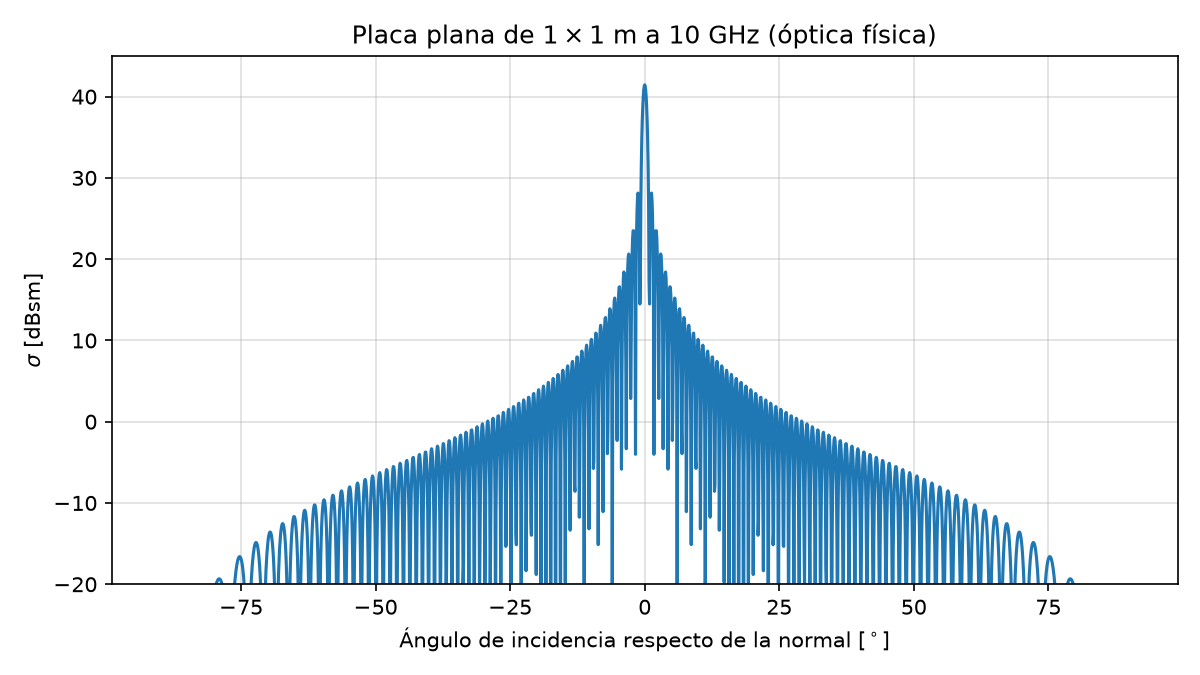
\includegraphics[width=0.75\textwidth]{teoria/rcs_placa.png}
    \caption{RCS de una placa plana cuadrada en función del ángulo de incidencia (aproximación de óptica física). Elaboración propia.}
    \label{fig:rcs_placa}
\end{figure}

\textbf{Blancos complejos.} Un avión o un barco se comportan como un conjunto de dispersores (bordes, cavidades, superficies, motores) cuyos ecos se suman con fases que cambian con el ángulo, por lo que su RCS varía decenas de dB con pequeñas rotaciones. Sus perfiles de RCS en función del ángulo de aspecto se obtienen \cite{apunte, skolnik}:
\begin{itemize}
    \item \underline{Por medición:} en polígonos al aire libre con el blanco en escala real montado sobre columnas de espuma o de metal de baja reflexión; en cámaras anecoicas de campo compacto; o con modelos a escala, escalando la longitud de onda en el mismo factor que las dimensiones ($\sigma' = \sigma/S^2$).
    \item \underline{Por cálculo electromagnético:} métodos de alta frecuencia (óptica física y teoría física de la difracción), eficientes para geometrías grandes y suaves, o métodos numéricos exactos como el método de los momentos, de mayor costo computacional. También se descompone el blanco en formas simples de RCS conocida.
\end{itemize}
Como la RCS de un blanco real fluctúa, para el diseño se describe estadísticamente con los modelos de Swerling, que definen su función de densidad y la rapidez de su variación (de exploración a exploración o de pulso a pulso) \cite{apunte}.

% =====================================================================
\subsection{Filtro apareado}
\label{sec:filtro_apareado}

\textbf{Definición.} El filtro apareado es el filtro lineal que maximiza la relación señal a ruido en un instante de muestreo $t_0$ cuando a la señal conocida $s(t)$ se le suma ruido \cite{skolnik, richards}.

\textbf{Derivación con ruido blanco gaussiano (AWGN).} Sea $x(t) = s(t) + n(t)$, con $n(t)$ de densidad espectral bilateral $N_0/2$, aplicada a un filtro $H(f)$. La señal de salida en $t_0$ y la potencia media del ruido de salida son
\begin{equation}
    y_s(t_0) = \int_{-\infty}^{\infty} H(f) S(f) e^{j2\pi f t_0} \, df,
    \qquad
    \overline{n_o^2} = \frac{N_0}{2} \int_{-\infty}^{\infty} |H(f)|^2 \, df
\end{equation}
Por la desigualdad de Schwarz, $\left| \int H S e^{j2\pi f t_0} df \right|^2 \leq \int |H|^2 df \cdot \int |S|^2 df$, de modo que
\begin{equation}
    SNR(t_0) = \frac{|y_s(t_0)|^2}{\overline{n_o^2}} \leq \frac{\int |S(f)|^2 df}{N_0/2} = \frac{2E}{N_0}
\end{equation}
donde $E$ es la energía de la señal. La igualdad se cumple cuando el filtro es
\begin{equation}
    H(f) = K \, S^*(f) \, e^{-j2\pi f t_0}
    \qquad \Longleftrightarrow \qquad
    h(t) = K \, s^*(t_0 - t)
    \label{eq:matched}
\end{equation}
Su respuesta en frecuencia tiene el mismo módulo que el espectro de la señal y la fase opuesta, más un retardo; su respuesta al impulso es la señal invertida en el tiempo y conjugada. La salida es la autocorrelación de la señal centrada en $t_0$:
\begin{equation}
    y(t) = K \int_{-\infty}^{\infty} s(\tau) \, s^*(\tau - t + t_0) \, d\tau = K \, R_{ss}(t - t_0)
\end{equation}

\textbf{Propiedades principales} \cite{apunte, richards}:
\begin{itemize}
    \item La SNR máxima, $2E/N_0$, depende solo de la energía de la señal y no de su forma. Un pulso largo modulado puede tener la misma SNR que uno corto de mayor potencia pico.
    \item $|H(f)| = |S(f)|$: el filtro da más peso a las frecuencias donde la señal tiene más energía.
    \item El ancho del pico de salida es del orden de $1/B$, la inversa del ancho de banda de la señal, y no de su duración. Esto es la base de la compresión de pulsos (\autoref{sec:chirp}).
    \item Con un pulso rectangular simple, el filtro apareado equivale a un filtro pasabanda con $B\tau \approx 1$.
\end{itemize}
En radar es importante porque maximiza la detectabilidad para un umbral dado (máxima $P_d$ para una $P_{fa}$ fija) y, con formas de onda moduladas, combina la energía de un pulso largo con la resolución de uno corto. Es además el procesamiento que se realiza en la práctica de este trabajo.

\textbf{Ruido no blanco.} Si el ruido tiene densidad espectral $N_i(f)$ no constante, el filtro óptimo es \cite{apunte, skolnik}
\begin{equation}
    H(f) = K \, \frac{S^*(f)}{N_i(f)} \, e^{-j2\pi f t_0}
\end{equation}
que equivale a un filtro blanqueador $1/\sqrt{N_i(f)}$ seguido del filtro apareado a la señal blanqueada. Un filtro apareado diseñado para AWGN pierde SNR en estos casos, y cuánto pierde depende de cuánto se superpone el espectro del ruido con el de la señal. Ejemplos:
\begin{itemize}
    \item \underline{Clutter:} su espectro Doppler se concentra cerca de cero (tierra) o alrededor de la velocidad del viento (lluvia, chaff). Los canceladores MTI y el filtrado Doppler actúan como el blanqueamiento en tiempo lento.
    \item \underline{Interferencia de banda angosta o \textit{jamming}:} concentra la potencia en parte de la banda. El filtro óptimo atenúa esas frecuencias (filtro de ranura o \textit{notch}).
    \item \underline{Ruido de fase y ruido no gaussiano:} por ejemplo, los picos de clutter de mar, que hacen que la estadística del umbral deje de ser de Rayleigh y aumenten las falsas alarmas.
\end{itemize}
En la práctica también se usan desajustes deliberados: ponderar el filtro con una ventana (Hamming, Taylor) baja los lóbulos laterales en rango a costa de 1 a 1,5 dB de pérdida de SNR y de un pico más ancho \cite{richards}.

% =====================================================================
\subsection{Clutter}
\label{sec:clutter}

\textbf{Definición.} El clutter es el conjunto de ecos no deseados que el radar recibe de objetos que no son los blancos de interés: el suelo, el mar, la lluvia, las aves o el chaff \cite{skolnik, apunte}. A diferencia del ruido térmico, es un eco de la propia señal transmitida: crece con la potencia transmitida y suele estar correlacionado entre pulsos. Su nivel puede superar en 50 o 60 dB al del blanco. Se caracteriza por su coeficiente de retrodispersión, por unidad de área ($\sigma^0$, para superficies) o de volumen ($\eta$), y por su espectro Doppler.

\textbf{Tipos y ejemplos} \cite{apunte, skolnik}:
\begin{itemize}
    \item \underline{Clutter de superficie terrestre:} terreno, edificios, árboles y montañas. Su valor medio es grande ($\sigma^0 \approx -20$ dB es típico) y su espectro Doppler es angosto y centrado en cero para un radar fijo, ensanchado por la vegetación movida por el viento. Por ejemplo, para un radar de vigilancia aérea con celda de 100 m, haz de $1{,}5^\circ$ y $R = 60$ km resulta $\sigma_{clutter} \approx 1500$ m$^2$, y para detectar un avión de 1 m$^2$ hace falta suprimirlo unos 45 dB \cite{apunte}.
    \item \underline{Clutter de mar:} unas 100 veces menor que el de tierra, depende del estado del mar, el viento, la polarización y el ángulo rasante. Con ángulos rasantes bajos aparecen picos (\textit{sea spikes}) que generan falsas alarmas.
    \item \underline{Clutter volumétrico meteorológico:} lluvia, nieve y granizo. Su reflectividad crece con $f^4$, por lo que es un problema en banda S y crítico en X y bandas superiores, y casi no afecta en banda L. Se mueve con el viento, por lo que tiene corrimiento y dispersión Doppler.
    \item \underline{Chaff:} nubes de dipolos metálicos de $\lambda/2$ lanzadas como contramedida; producen ecos intensos ($\sigma \approx 0{,}18\lambda^2$ por dipolo) que se desplazan con el viento.
    \item \underline{Clutter biológico (``ángeles''):} aves e insectos. Tienen RCS pequeña pero, en bandadas o enjambres, generan falsas alarmas; como son lentos, se filtran por velocidad.
    \item \underline{Clutter puntual o discreto:} torres, edificios altos, aerogeneradores (con Doppler por el giro de las palas) y vehículos en rutas.
\end{itemize}
Según la geometría se clasifica también en clutter de lóbulo principal, de lóbulos laterales y de altitud (el suelo justo debajo de un radar aerotransportado). En la señal del trabajo práctico se observa clutter a corta distancia, en torno a 1,8 km, que aparece en todas las señales y se elimina con el cancelador MTI.

% =====================================================================
\subsection{Señal chirp y compresión de pulsos}
\label{sec:chirp}

\textbf{Definición.} Un chirp es un pulso de duración $T$ con modulación lineal de frecuencia (LFM): su frecuencia instantánea recorre linealmente un ancho de banda $B$ durante el pulso \cite{richards, cumming}. En banda base,
\begin{equation}
    s(t) = \mathrm{rect}\left(\frac{t}{T}\right) e^{j\pi \frac{B}{T} t^2},
    \qquad
    f_i(t) = \frac{1}{2\pi}\frac{d\phi}{dt} = \frac{B}{T} \, t
\end{equation}
La sigla \textit{Compressed High Intensity Radar Pulse} resume su propósito: transmitir un pulso largo y de potencia moderada que, al recibirlo, se comprime en un pico angosto e intenso.

\textbf{Por qué interesa en radar.} En un pulso simple hay un compromiso: la energía, y con ella el alcance (\autoref{eq:snr}), crece con la duración del pulso, pero la resolución en rango empeora, $\Delta R = c T/2$. Los transmisores tienen una potencia pico limitada, por lo que no se puede acortar el pulso sin perder energía. El chirp desacopla ambas cosas: la energía depende de $T$ y la resolución, de $B$ \cite{apunte, richards}. Además, el chirp es tolerante al Doppler, aunque con un acoplamiento rango-Doppler: un corrimiento Doppler desplaza levemente el pico comprimido.

\textbf{Proceso de compresión.} El receptor aplica el filtro apareado $h(t) = s^*(-t)$ (\autoref{eq:matched}), que en frecuencia multiplica por $S^*(f)$ y compensa la fase cuadrática del chirp: todas las componentes de frecuencia se alinean en el mismo instante. Para $BT \gg 1$ la salida es aproximadamente \cite{richards, cumming}
\begin{equation}
    y(t) \approx T \, \mathrm{sinc}(B t) = T \, \frac{\sin(\pi B t)}{\pi B t}
\end{equation}
un pico de ancho $\approx 1/B$ (entre ceros, $2/B$). La relación entre la duración del pulso transmitido y la del comprimido es la \textbf{relación de compresión}, igual al producto tiempo-ancho de banda $BT$. En amplitud, el pico crece en $\sqrt{BT}$ y la SNR en $BT$ veces respecto del pulso sin comprimir. Los lóbulos laterales de la sinc quedan a $-13{,}2$ dB, y se reducen ponderando el filtro con una ventana a costa de ensanchar el pico \cite{richards}.

\textbf{Relación con la resolución.} Dos blancos se distinguen si sus picos comprimidos no se superponen, es decir, si están separados más que
\begin{equation}
    \Delta R = \frac{c}{2B}
\end{equation}
que depende solo del ancho de banda. En este trabajo, $T = 10 \, [\mu s]$ y $B = 2 \, [MHz]$, con $BT = 20$ (13 dB de ganancia de compresión): sin comprimir, la resolución sería de $cT/2 = 1500 \, [m]$, y comprimido es de $c/(2B) = 75 \, [m]$, 20 veces mejor (\autoref{fig:chirp}). Gracias a esto, en la práctica se separan blancos a 300 m de distancia, como los de 15,21 y 15,51 km de la señal 1.

\begin{figure}[H]
    \centering
    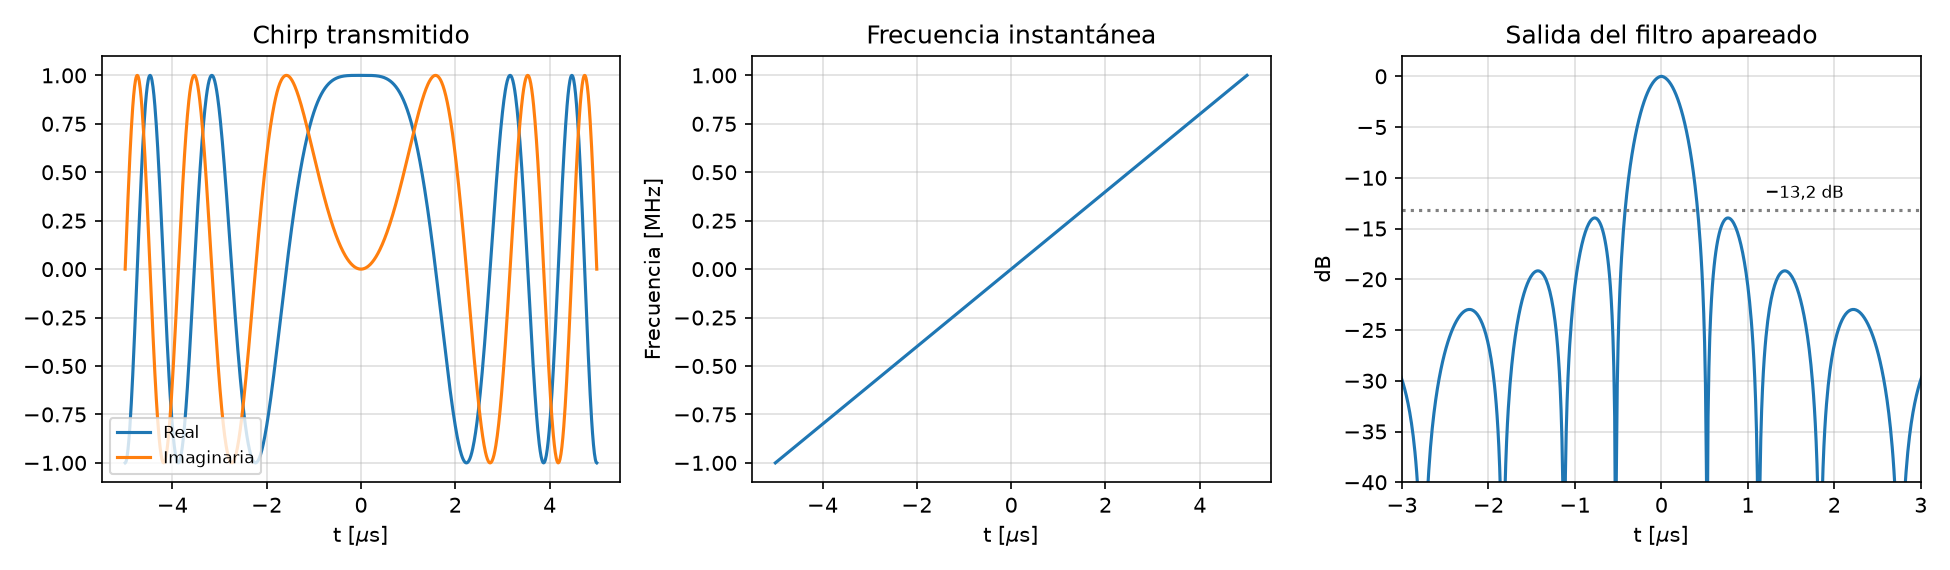
\includegraphics[width=\textwidth]{teoria/chirp_compresion.png}
    \caption{Chirp del trabajo práctico ($T = 10 \, [\mu s]$, $B = 2 \, [MHz]$), su frecuencia instantánea y la salida del filtro apareado. Con $BT = 20$ el primer lóbulo lateral queda en $-14{,}0$ dB, próximo al valor de $-13{,}2$ dB de la sinc ideal. Elaboración propia.}
    \label{fig:chirp}
\end{figure}

\newpage
\section{Parte práctica: procesamiento de la señal \senal}
\label{sec:practico}

\subsection{Datos y parámetros del radar}
\label{sec:parametros}
La señal asignada (\texttt{signal\_\senal.csv}) es una detección simulada de radar con 100 momentos de muestreo, es decir, 100 pulsos consecutivos, con entre 2 y 10 blancos de rangos y velocidades desconocidos \cite{consigna}. Cada pulso tiene 2000 muestras complejas (I/Q) de tiempo rápido, que cubren de 15 m a 30 km con un paso de $c\,t_s/2 = 15 \, [m]$. Los datos se ordenan en una matriz de $100 \times 2000$: las filas son el \textbf{tiempo lento} (pulso a pulso, separados una PRI) y las columnas el \textbf{tiempo rápido} (rango). Se procesaron en Python (\texttt{numpy}, \texttt{scipy}, \texttt{matplotlib}) a partir del código provisto por la cátedra \cite{codigo_catedra}. El script \texttt{practico/tp5\_radar.py} reproduce todos los resultados con \texttt{python tp5\_radar.py \senal}.

\begin{table}[H]
    \centering
    \footnotesize
    \caption{Parámetros del radar simulado \cite{codigo_catedra} y magnitudes derivadas.}
    \label{tab:parametros}
    \begin{tabular}{|l|r||l|r|}
        \hline
        \textbf{Parámetro} & \textbf{Valor} & \textbf{Magnitud derivada} & \textbf{Valor} \\
        \hline
        Frecuencia portadora $f_c$ & 1,3 GHz & Longitud de onda $\lambda = c/f_c$ & 23,1 cm \\
        Frecuencia de muestreo $f_s$ & 10 MHz & Paso en rango $c/(2f_s)$ & 15 m \\
        Duración del chirp $T_p$ & 10 $\mu$s & Resolución en rango $c/(2B)$ & 75 m \\
        Ancho de banda del chirp $B$ & 2 MHz & Producto $BT$ (ganancia de compresión) & 20 (13 dB) \\
        PRF & 1500 Hz & PRI & 666,7 $\mu$s \\
        Recuperación del transmisor $T_e$ & 5 $\mu$s & Rango mínimo $(T_p/2 + T_e)c/2$ & 1,5 km \\
        Pulsos $N_p$ & 100 & Rango no ambiguo $c(PRI - T_p - T_e)/2$ & 97,75 km \\
        Ventana de rango & 30 km & Intervalo de velocidad no ambigua $\pm \lambda\,PRF/4$ & $\pm 86{,}5$ m/s \\
        \hline
    \end{tabular}
\end{table}

\subsection{Operaciones realizadas}
\label{sec:operaciones}
La \autoref{fig:flujo} resume la cadena de procesamiento, que sigue el diagrama de la consigna \cite{consigna}.

\begin{figure}[H]
    \centering
    \resizebox{\textwidth}{!}{%
    \begin{tikzpicture}[font=\footnotesize, node distance=0.5cm and 0.6cm,
        b/.style={draw, thick, rounded corners=2pt, fill=blue!8, minimum height=0.9cm, text width=2.1cm, align=center},
        f/.style={-{Stealth}, thick}]
        \node[b] (raw) {Datos crudos $100 \times 2000$};
        \node[b, right=of raw] (mf) {Filtro apareado (compresión)};
        \node[b, right=1.0cm of mf, fill=orange!12] (sti) {STI SC $1 + z^{-1}$};
        \node[b, above=of sti, fill=orange!12] (mti) {MTI SC $1 - z^{-1}$};
        \node[b, below=of sti, fill=orange!12] (dc) {MTI DC $1 - 2z^{-1} + z^{-2}$};
        \node[b, right=of mti, fill=green!10] (dop) {Filtrado Doppler (DFT en tiempo lento)};
        \node[b, right=of sti, fill=green!10] (cfar) {CFAR y cruces por cero};
        \node[b, right=of dop, fill=purple!10] (vel) {Rango y velocidad de blancos móviles};
        \node[b, right=of cfar, fill=purple!10] (rng) {Rango de los blancos (móviles y fijos)};
        \draw[f] (raw) -- (mf); \draw[f] (mf) -- (sti); \draw[f] (mf.east) -- ++(0.4,0) |- (mti); \draw[f] (mf.east) -- ++(0.4,0) |- (dc);
        \draw[f] (mti) -- (dop); \draw[f] (dop) -- (vel); \draw[f] (sti) -- (cfar); \draw[f] (cfar) -- (rng);
        \draw[f] (mti.east) -- ++(0.25,0) |- (cfar); \draw[f] (dc.east) -- ++(0.25,0) |- (cfar);
    \end{tikzpicture}}
    \caption{Cadena de procesamiento implementada.}
    \label{fig:flujo}
\end{figure}

\textbf{1. Compresión con filtro apareado.} Se genera el chirp de referencia $s(t) = \mathrm{rect}(t/T_p) \, e^{j\pi (B/T_p) t^2}$ y el filtro apareado $h(t) = s^*(-t)$ (\autoref{sec:filtro_apareado}). Cada pulso recibido $x_p[n]$ se convoluciona con $h$ mediante la FFT (función \texttt{fastconv} de la cátedra, con relleno de ceros a la potencia de 2 siguiente):
\begin{equation}
    y_p[n] = \sum_k x_p[k] \, h[n - k] = \mathrm{IFFT}\{ X_p(f) \, S^*(f) \}
\end{equation}
La salida de la convolución tiene $2 \cdot 2000 - 1$ muestras. Se conservan las 2000 centrales, a partir del índice $(N_h - 1)/2$, para que el pico de cada eco coincida con su rango. La alineación se verificó con un eco sintético a 10 km, cuyo pico comprimido aparece exactamente en $10{,}005$ km, la celda de 15 m que lo contiene.

\textbf{2. Canceladores en tiempo lento.} Operan sobre la señal comprimida, celda de rango por celda de rango, entre pulsos consecutivos:
\begin{align}
    \text{MTI simple cancelador:} \quad & y_p = x_p - x_{p-1}, & H(z) &= 1 - z^{-1}, & |H(f_D)| &= 2\left|\sin(\pi f_D / PRF)\right| \\
    \text{STI simple cancelador:} \quad & y_p = x_p + x_{p-1}, & H(z) &= 1 + z^{-1}, & |H(f_D)| &= 2\left|\cos(\pi f_D / PRF)\right| \\
    \text{MTI doble cancelador:} \quad & y_p = x_p - 2x_{p-1} + x_{p-2}, & H(z) &= (1 - z^{-1})^2, & |H(f_D)| &= 4\sin^2(\pi f_D / PRF)
\end{align}
con $f_D = 2v_r/\lambda$. El MTI es un filtro pasaaltos en Doppler: anula los ecos fijos (clutter y blancos detenidos) y deja pasar los móviles. El doble cancelador tiene un nulo más ancho y profundo alrededor de $f_D = 0$, mejor para clutter con dispersión Doppler, pero atenúa más a los blancos lentos. El STI es pasabajos: refuerza los ecos fijos y anula los blancos cuya $f_D$ se acerca a $\pm PRF/2$. Todos se repiten cada $PRF$: un blanco con velocidad $v_b = k \lambda \, PRF/2 = k \cdot 173 \, [m/s]$ (velocidad ciega) es cancelado por el MTI como si estuviera fijo (\autoref{fig:canceladores}).

\begin{figure}[H]
    \centering
    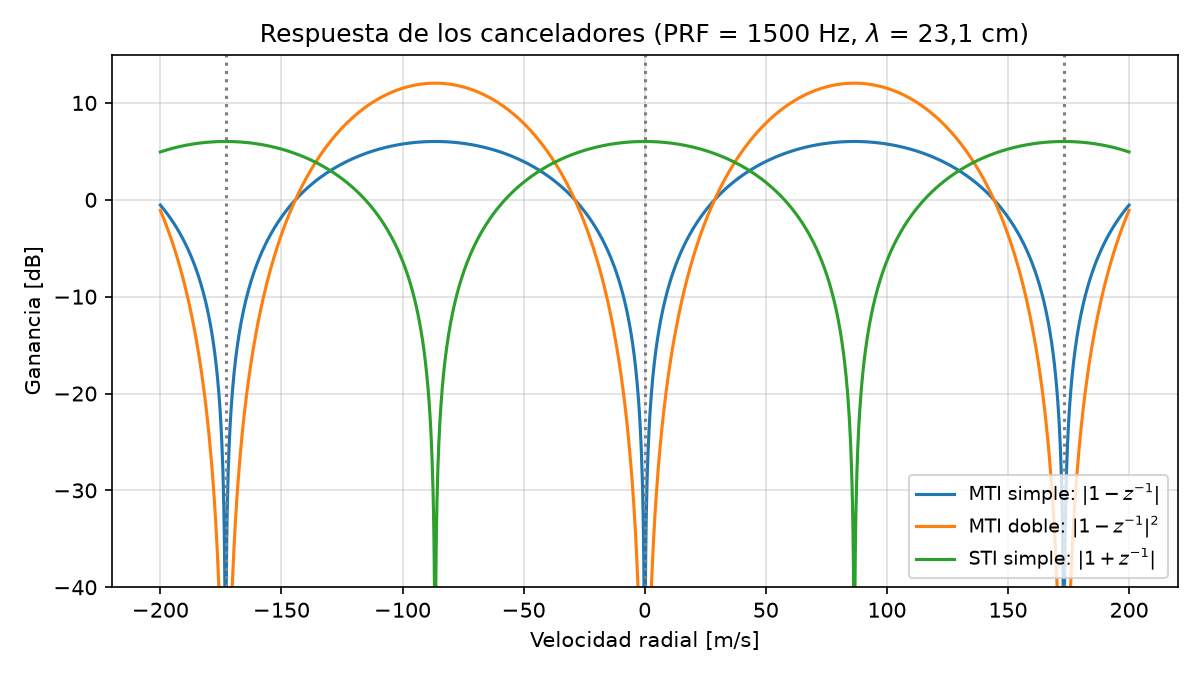
\includegraphics[width=0.78\textwidth]{teoria/respuesta_canceladores.png}
    \caption{Respuesta en frecuencia de los canceladores en función de la velocidad radial. Las líneas punteadas marcan la velocidad nula y las velocidades ciegas $\pm 173 \, [m/s]$. Elaboración propia.}
    \label{fig:canceladores}
\end{figure}

\textbf{3. Ventana CFAR y umbral.} Se usa un detector CA-CFAR (\textit{cell averaging}): para cada celda bajo prueba se estima la potencia de ruido como el promedio de $N_R$ celdas de referencia, dejando $N_G$ celdas de guarda a cada lado para que el propio blanco no eleve la estimación \cite{apunte, richards}. Implementado como convolución con la ventana $w$ (\autoref{fig:ventana_cfar}),
\begin{equation}
    \hat{P}[n] = \sum_k w[k] \, |y[n-k]|^2,
    \qquad
    w[k] = \begin{cases} 1/N_R & \text{celdas de referencia} \\ 0 & \text{celdas de guarda y celda bajo prueba} \end{cases}
\end{equation}
y se declara detección cuando $|y[n]|^2 > \alpha \, \hat{P}[n]$. Para ruido gaussiano complejo detectado en potencia, la $P_{fa}$ de diseño fija el factor del umbral \cite{richards}:
\begin{equation}
    P_{fa} = \left(1 + \frac{\alpha}{N_R}\right)^{-N_R}
    \quad \Rightarrow \quad
    \alpha = N_R \left( P_{fa}^{-1/N_R} - 1 \right)
\end{equation}
Se adoptaron $N_R = 64$ celdas de referencia (32 de cada lado, 480 m) y $N_G = 8$ celdas de guarda por lado (120 m), con $P_{fa} = 10^{-6}$:
\begin{itemize}
    \item $\alpha = 15{,}4$, que en amplitud corresponde a una \textbf{ganancia del umbral de $\sqrt{\alpha} = 3{,}93$} sobre el valor eficaz del ruido estimado.
    \item Las celdas de guarda cubren el lóbulo principal del eco comprimido ($\pm 75$ m, 5 celdas) y sus primeros lóbulos laterales ($\pm 110$ m), para que el blanco no se cuente como ruido.
    \item El ejemplo de la consigna usa 200 celdas de referencia (1,5 km por lado). Con esa ventana se verificó enmascaramiento: un blanco fuerte dentro de la ventana de otro eleva su umbral y lo oculta (con la señal 2, el blanco fijo de 22,02 km quedaba oculto por los de 20,2--20,3 km). La ventana de 64 celdas reduce ese efecto con una pérdida CFAR moderada.
    \item En los extremos del vector de rango hay menos celdas de referencia; el promedio se normaliza por las celdas disponibles para que el umbral no caiga artificialmente en los bordes.
\end{itemize}

\begin{figure}[H]
    \centering
    \includegraphics[width=0.55\textwidth]{\figdir/03_ventana_cfar.png}
    \caption{Ventana CFAR utilizada: 64 celdas de referencia (32 por lado, con valor $1/64$), 8 celdas de guarda por lado y la celda bajo prueba en el centro (valor 0).}
    \label{fig:ventana_cfar}
\end{figure}

\textbf{4. Detección por cruces por cero.} La función $d[n] = \mathrm{sign}(|y[n]| - V_T[n])$ vale $+1$ donde la señal supera el umbral. Su diferencia, $\Delta d[n] = d[n+1] - d[n]$ (funciones \texttt{numpy.sign} y \texttt{numpy.diff}), vale $+2$ donde comienza una detección y $-2$ donde termina. El rango del blanco es el del máximo de $|y|$ dentro de cada intervalo. Las detecciones a menos de 150 m (dos celdas de resolución) se agrupan, porque corresponden al mismo eco y sus lóbulos laterales. Se descartan las celdas por debajo del rango mínimo de 1,5 km.

Los gráficos CFAR usan, como pide la consigna, un único momento de muestreo: los pulsos $t_0$ y $t_1$ para los canceladores simples y $t_0$, $t_1$ y $t_2$ para el doble. Para una lista de detecciones más robusta se aplica además el CFAR a la potencia de la salida de cada cancelador promediada sobre todos los pulsos (integración no coherente).

\textbf{5. Filtrado Doppler.} La señal del MTI simple cancelador (99 pulsos $\times$ 2000 celdas) se multiplica, transpuesta, por la matriz de la DFT de $m = 99$ puntos \cite{consigna}:
\begin{equation}
    \mathbf{Y} = (\mathbf{MTI}_{SC})^T \, \mathbf{F_D},
    \qquad
    F_D[r, c] = e^{-j 2\pi r c / m}, \quad r, c = 0, \dots, m-1
\end{equation}
Cada fila de $\mathbf{Y}$ es el espectro Doppler de una celda de rango, que integra coherentemente los 99 pulsos. La columna $k$ (centrada con \texttt{fftshift}) corresponde a $f_D = (k - m/2) \, PRF/m$ y a la velocidad radial $v_r = f_D \lambda/2$, con una resolución de $\lambda \, PRF/(2m) = 1{,}75 \, [m/s]$. Con la convención de fase del simulador ($e^{-jk \, 2R}$), una velocidad positiva corresponde a un blanco que se acerca y una negativa, a uno que se aleja. Las velocidades solo son únicas dentro de $\pm 86{,}5 \, [m/s]$: un blanco más rápido aparece replegado (\textit{aliasing}).

Para obtener la lista de blancos, sobre el mapa rango-Doppler se aplica el mismo CA-CFAR en rango para cada frecuencia Doppler. Para esa detección se pondera el tiempo lento con una ventana de Hamming, que baja los lóbulos laterales Doppler de $-13$ a $-43$ dB; sin ella, junto a cada blanco de unos 40 dB de SNR aparecían decenas de detecciones falsas en otras velocidades. Esta detección tiene dos ventajas: la integración coherente de 99 pulsos (casi 20 dB de ganancia) y la separación de blancos cercanos en rango pero con distinta velocidad, que ya no se enmascaran entre sí.

\textbf{6. Clasificación de los blancos.} Las detecciones se combinan con estos criterios:
\begin{itemize}
    \item \underline{Blanco móvil:} detección rango-Doppler confirmada por algún cancelador a menos de 150 m, o con SNR de al menos 20 dB. Su velocidad es la del máximo Doppler.
    \item \underline{Residuo:} una detección en la misma celda de rango que otra más de 20 dB más fuerte corresponde a la dispersión Doppler del blanco fuerte, por la fluctuación de su RCS entre pulsos, y no se cuenta como blanco.
    \item \underline{Falsa alarma:} una detección débil (SNR menor que 20 dB) que ningún cancelador confirma. En las señales 1, 2 y de ejemplo aparecen las mismas tres (1,5, 6,2 y 13,7 km), lo que indica que las simulaciones comparten la realización del ruido.
    \item \underline{Blanco fijo:} detección del STI integrado donde la salida del STI supera a la del MTI en más de 10 dB, porque el MTI cancela casi toda su energía.
\end{itemize}

\textbf{Validación.} El procedimiento se probó con la señal de ejemplo (\texttt{signal\_example.csv}). Se detectan tres blancos móviles en 10,02, 15,02 y 20,01 km, que coinciden con los de la Figura 5 de la consigna (9,95, 14,97 y 19,93 km), y un blanco fijo en 18,02 km, que solo aparece sin cancelar.

\subsection{Resultados de la señal 2}
\label{sec:resultados}

\subsubsection{Señal recibida y compresión}
La \autoref{fig:recibida} muestra un momento de muestreo (el pulso $t_0$). Hasta el rango mínimo de 1,5 km la señal es nula, porque el receptor está bloqueado durante la transmisión y la recuperación. Entre 1,5 y 2,5 km aparece un eco intenso, de hasta $8{,}0 \times 10^{-6}$, que corresponde a clutter cercano. Más allá, los ecos de los blancos quedan casi ocultos en el ruido. Solo se insinúa un aumento de nivel en torno a 20 km, donde se superponen varios ecos intensos, porque un chirp de 10 $\mu$s extiende cada eco sobre 1,5 km.

\begin{figure}[H]
    \centering
    \includegraphics[width=0.85\textwidth]{\figdir/01_senal_recibida.png}
    \caption{Señal 2: un momento de muestreo de la señal recibida. Arriba, partes real e imaginaria; abajo, módulo, en función del rango.}
    \label{fig:recibida}
\end{figure}

Después del filtro apareado (\autoref{fig:compresion}), la energía de cada eco se concentra en un pico de unos 75 m y emergen los blancos, entre 8 y 26,2 km. La zona de 20 km se resuelve en picos a 19,82 km y a 20,2--20,3 km. Los ecos de 20,22 y 20,31 km están a solo 90 m, apenas por encima de la resolución de 75 m. En la señal comprimida se ven como un pico ensanchado, y es el procesamiento en tiempo lento el que los separa: uno se mueve y el otro está fijo.

\begin{figure}[H]
    \centering
    \includegraphics[width=0.85\textwidth]{\figdir/02_compresion.png}
    \caption{Señal 2: módulo de la señal sin comprimir (arriba) y comprimida con el filtro apareado (abajo) para el mismo momento de muestreo.}
    \label{fig:compresion}
\end{figure}

\subsubsection{Canceladores y CFAR}
Las figuras \ref{fig:cfar_mti} a \ref{fig:cfar_mtidc} muestran, para cada cancelador:
\begin{itemize}
    \item las señales sin comprimir de los momentos de muestreo que usa;
    \item las señales comprimidas;
    \item la salida del cancelador con el umbral CFAR (ganancia 3,93);
    \item los cruces por cero que marcan el inicio ($+2$) y el fin ($-2$) de cada detección.
\end{itemize}

\begin{figure}[H]
    \centering
    \includegraphics[width=0.88\textwidth]{\figdir/04_cfar_mti_sc.png}
    \caption{Señal 2: CFAR del MTI simple cancelador ($x_1 - x_0$).}
    \label{fig:cfar_mti}
\end{figure}

\begin{figure}[H]
    \centering
    \includegraphics[width=0.88\textwidth]{\figdir/05_cfar_sti_sc.png}
    \caption{Señal 2: CFAR del STI simple cancelador ($x_1 + x_0$).}
    \label{fig:cfar_sti}
\end{figure}

\begin{figure}[H]
    \centering
    \includegraphics[width=0.88\textwidth]{\figdir/06_cfar_mti_dc.png}
    \caption{Señal 2: CFAR del MTI doble cancelador ($x_2 - 2x_1 + x_0$).}
    \label{fig:cfar_mtidc}
\end{figure}

\begin{table}[H]
    \centering
    \footnotesize
    \caption{Señal 2: rangos detectados por cada cancelador [km].}
    \label{tab:det_canceladores}
    \begin{tabular}{|l|p{6.2cm}|p{5.2cm}|}
        \hline
        \textbf{Cancelador} & \textbf{Un momento de muestreo ($t_0$, $t_1$, $t_2$)} & \textbf{Integrado sobre todos los pulsos} \\
        \hline
        MTI simple & 8,01 -- 12,02 -- 20,22 -- 26,23 & 8,01 -- 12,02 -- 20,22 -- 26,23 \\
        \hline
        STI simple & 8,01 -- 12,02 -- 15,62 -- 20,32 -- 22,02 & 8,01 -- 12,02 -- 15,62 -- 20,31 -- 22,02 \\
        \hline
        MTI doble & 8,03 -- 12,02 -- 20,20 -- 26,23 & 8,01 -- 12,02 -- 20,22 -- 26,23 \\
        \hline
    \end{tabular}
\end{table}

\textbf{Análisis:}
\begin{itemize}
    \item \underline{MTI simple y doble:} detectan cuatro blancos móviles (8,01, 12,02, 20,22 y 26,23 km). Cancelan el clutter cercano y los ecos fijos de 15,62, 20,31 y 22,02 km.
    \item \underline{STI simple:} refuerza los ecos fijos y detecta los tres blancos fijos, además de los móviles de 8,01 y 12,02 km. No detecta el de 26,23 km: su frecuencia Doppler ($+742$ Hz) está a menos de 8 Hz de $PRF/2$, donde el STI tiene su nulo (unos 30 dB de atenuación, \autoref{fig:canceladores}).
    \item \underline{Enmascaramiento:} el blanco de 19,82 km tiene una de las mayores SNR de la escena, pero ningún cancelador lo detecta. Está a 400 m de los ecos de 20,2--20,3 km, que caen dentro de su ventana de referencia y elevan el umbral CFAR (se ve el pico bajo el umbral en la \autoref{fig:cfar_sti}). Con la ventana de 200 celdas del ejemplo de la consigna el efecto era mayor: además se perdía el blanco fijo de 22,02 km. El procesamiento Doppler lo separa, porque tiene otra velocidad.
\end{itemize}

\subsubsection{Procesamiento Doppler}
La \autoref{fig:doppler3d} es el gráfico 3D del producto Doppler de la señal MTI: cada pico es un blanco móvil ubicado en su rango y su velocidad. La \autoref{fig:mapa} muestra la vista superior en dB con los blancos detectados. Allí se ve que los ecos de 19,82 y 20,22 km, cercanos en rango, quedan en velocidades distintas ($-24{,}5$ y $-43{,}7$ m/s).

\begin{figure}[H]
    \centering
    \includegraphics[width=0.85\textwidth]{\figdir/07_doppler_3d.png}
    \caption{Señal 2: procesamiento Doppler de la señal del MTI simple cancelador (módulo en función de la velocidad y el rango).}
    \label{fig:doppler3d}
\end{figure}

\begin{figure}[H]
    \centering
    \includegraphics[width=0.85\textwidth]{\figdir/08_mapa_rango_velocidad.png}
    \caption{Señal 2: mapa rango-velocidad en dB con los blancos móviles (cruces) y los blancos fijos, ubicados en velocidad nula (cuadrados).}
    \label{fig:mapa}
\end{figure}

\subsubsection{Blancos detectados}
La \autoref{tab:blancos} reúne el resultado final: \textbf{ocho blancos, cinco móviles y tres fijos}.

\begin{table}[H]
    \centering
    \footnotesize
    \caption{Señal 2: blancos detectados. La velocidad positiva indica acercamiento y la negativa, alejamiento. Las ganancias del MTI y el STI corresponden a la frecuencia Doppler de cada blanco.}
    \label{tab:blancos}
    \begin{tabular}{|c|r|r|r|r|r|r|r|l|}
        \hline
        \textbf{N.°} & \textbf{Rango [km]} & \textbf{$v_r$ [m/s]} & \textbf{$v_r$ [km/h]} & \textbf{$f_D$ [Hz]} & \textbf{SNR [dB]} & \textbf{MTI [dB]} & \textbf{STI [dB]} & \textbf{Tipo} \\
        \hline
        1 & 8,01 & $-31{,}5$ & $-113$ & $-273$ & 39,5 & $+0{,}7$ & $+4{,}5$ & Móvil \\
        2 & 12,02 & $-59{,}4$ & $-214$ & $-515$ & 40,6 & $+4{,}9$ & $-0{,}5$ & Móvil \\
        3 & 15,62 & 0 & 0 & 0 & -- & $-\infty$ & $+6{,}0$ & Fijo \\
        4 & 19,82 & $-24{,}5$ & $-88$ & $-212$ & 42,7 & $-1{,}3$ & $+5{,}1$ & Móvil \\
        5 & 20,22 & $-43{,}7$ & $-157$ & $-379$ & 42,1 & $+3{,}1$ & $+2{,}9$ & Móvil \\
        6 & 20,31 & 0 & 0 & 0 & -- & $-\infty$ & $+6{,}0$ & Fijo \\
        7 & 22,02 & 0 & 0 & 0 & -- & $-\infty$ & $+6{,}0$ & Fijo \\
        8 & 26,24 & $+85{,}7$ & $+308$ & $+742$ & 33,2 & $+6{,}0$ & $-29{,}9$ & Móvil (*) \\
        \hline
    \end{tabular}

    \vspace{0.1cm}
    \raggedright \scriptsize (*) Velocidad en el borde del intervalo no ambiguo ($\pm 86{,}5$ m/s): podría ser una velocidad replegada, por ejemplo $-87{,}4$ m/s, que difiere en $\lambda \, PRF/2 = 173$ m/s.
\end{table}

\begin{itemize}
    \item \underline{Blancos fijos:} los de 15,62, 20,31 y 22,02 km tienen una salida del STI entre 22 y 24 dB mayor que la del MTI. Son ecos sin Doppler, como blancos detenidos o reflectores fijos, que el MTI cancela. El de 20,31 km comparte casi la misma celda con el blanco móvil de 20,22 km: los distingue que el STI tiene su máximo en 20,31 km y el MTI en 20,22 km, con 24 dB más de salida en el STI.
    \item \underline{Residuos y falsas alarmas:} el mapa rango-Doppler tiene detecciones débiles en velocidad nula o casi nula a 8,03, 12,0 y 19,82 km. Son más de 20 dB menores que los blancos de esas celdas y corresponden a la dispersión Doppler por la fluctuación de su RCS. Además hay tres detecciones aisladas (1,5, 6,2 y 13,7 km) de unos 10 dB de SNR que ningún cancelador confirma. Todas se descartaron con los criterios de la \autoref{sec:operaciones}.
    \item \underline{Resolución en velocidad:} es de 1,75 m/s. Las velocidades informadas tienen una incertidumbre de media celda Doppler ($\pm 0{,}9$ m/s).
\end{itemize}


\section{Conclusiones}
\begin{itemize}
    \item En la señal 2 se identificaron \textbf{ocho blancos}:
    \begin{itemize}
        \item \underline{Cinco móviles:} 8,01 km a $-31{,}5$ m/s, 12,02 km a $-59{,}4$ m/s, 19,82 km a $-24{,}5$ m/s, 20,22 km a $-43{,}7$ m/s y 26,24 km a $+85{,}7$ m/s.
        \item \underline{Tres fijos:} 15,62, 20,31 y 22,02 km.
    \end{itemize}
    \item La compresión con filtro apareado fue imprescindible: en la señal cruda los ecos quedan ocultos en el ruido y extendidos sobre 1,5 km, mientras que comprimidos ganan 13 dB y se resuelven con 75 m de resolución.
    \item La zona de 20 km concentra tres blancos en 500 m: 19,82 km (móvil), 20,22 km (móvil) y 20,31 km (fijo). Los dos últimos, a 90 m, se distinguen porque uno sobrevive al MTI y el otro al STI. El de 19,82 km, enmascarado en el CFAR de todos los canceladores, solo se detecta en el mapa rango-Doppler, donde su velocidad lo separa de los vecinos.
    \item Los canceladores cumplen funciones complementarias. El MTI elimina el clutter cercano y los ecos fijos y deja los blancos móviles; el STI hace lo contrario; el MTI doble ensancha el nulo de velocidad cero. Sus nulos producen velocidades ciegas: el blanco de 26,24 km, con $f_D$ cerca de $PRF/2$, desaparece en el STI.
    \item El CA-CFAR mantiene la tasa de falsas alarmas adaptando el umbral al ruido local, pero los blancos intensos enmascaran a sus vecinos. Con la ventana de 200 celdas del ejemplo se perdía también el blanco fijo de 22,02 km; con 64 celdas de referencia y 8 de guarda por lado se recupera.
    \item El filtrado Doppler aporta la velocidad de cada blanco y la integración coherente de 99 pulsos (unos 20 dB), y fue el método de detección más robusto en esta escena congestionada.
    \item La PRF de 1500 Hz limita las velocidades no ambiguas a $\pm 86{,}5$ m/s: el blanco de 26,24 km está en el borde y su velocidad podría estar replegada. Para resolverlo haría falta una segunda PRF (PRF escalonada), como indica el apunte de la cátedra \cite{apunte}.
\end{itemize}

\newpage
\printbibliography[heading=bibintoc, title={Bibliografía y Referencias}]
\end{document}
